\begin{figure}
        \centering
        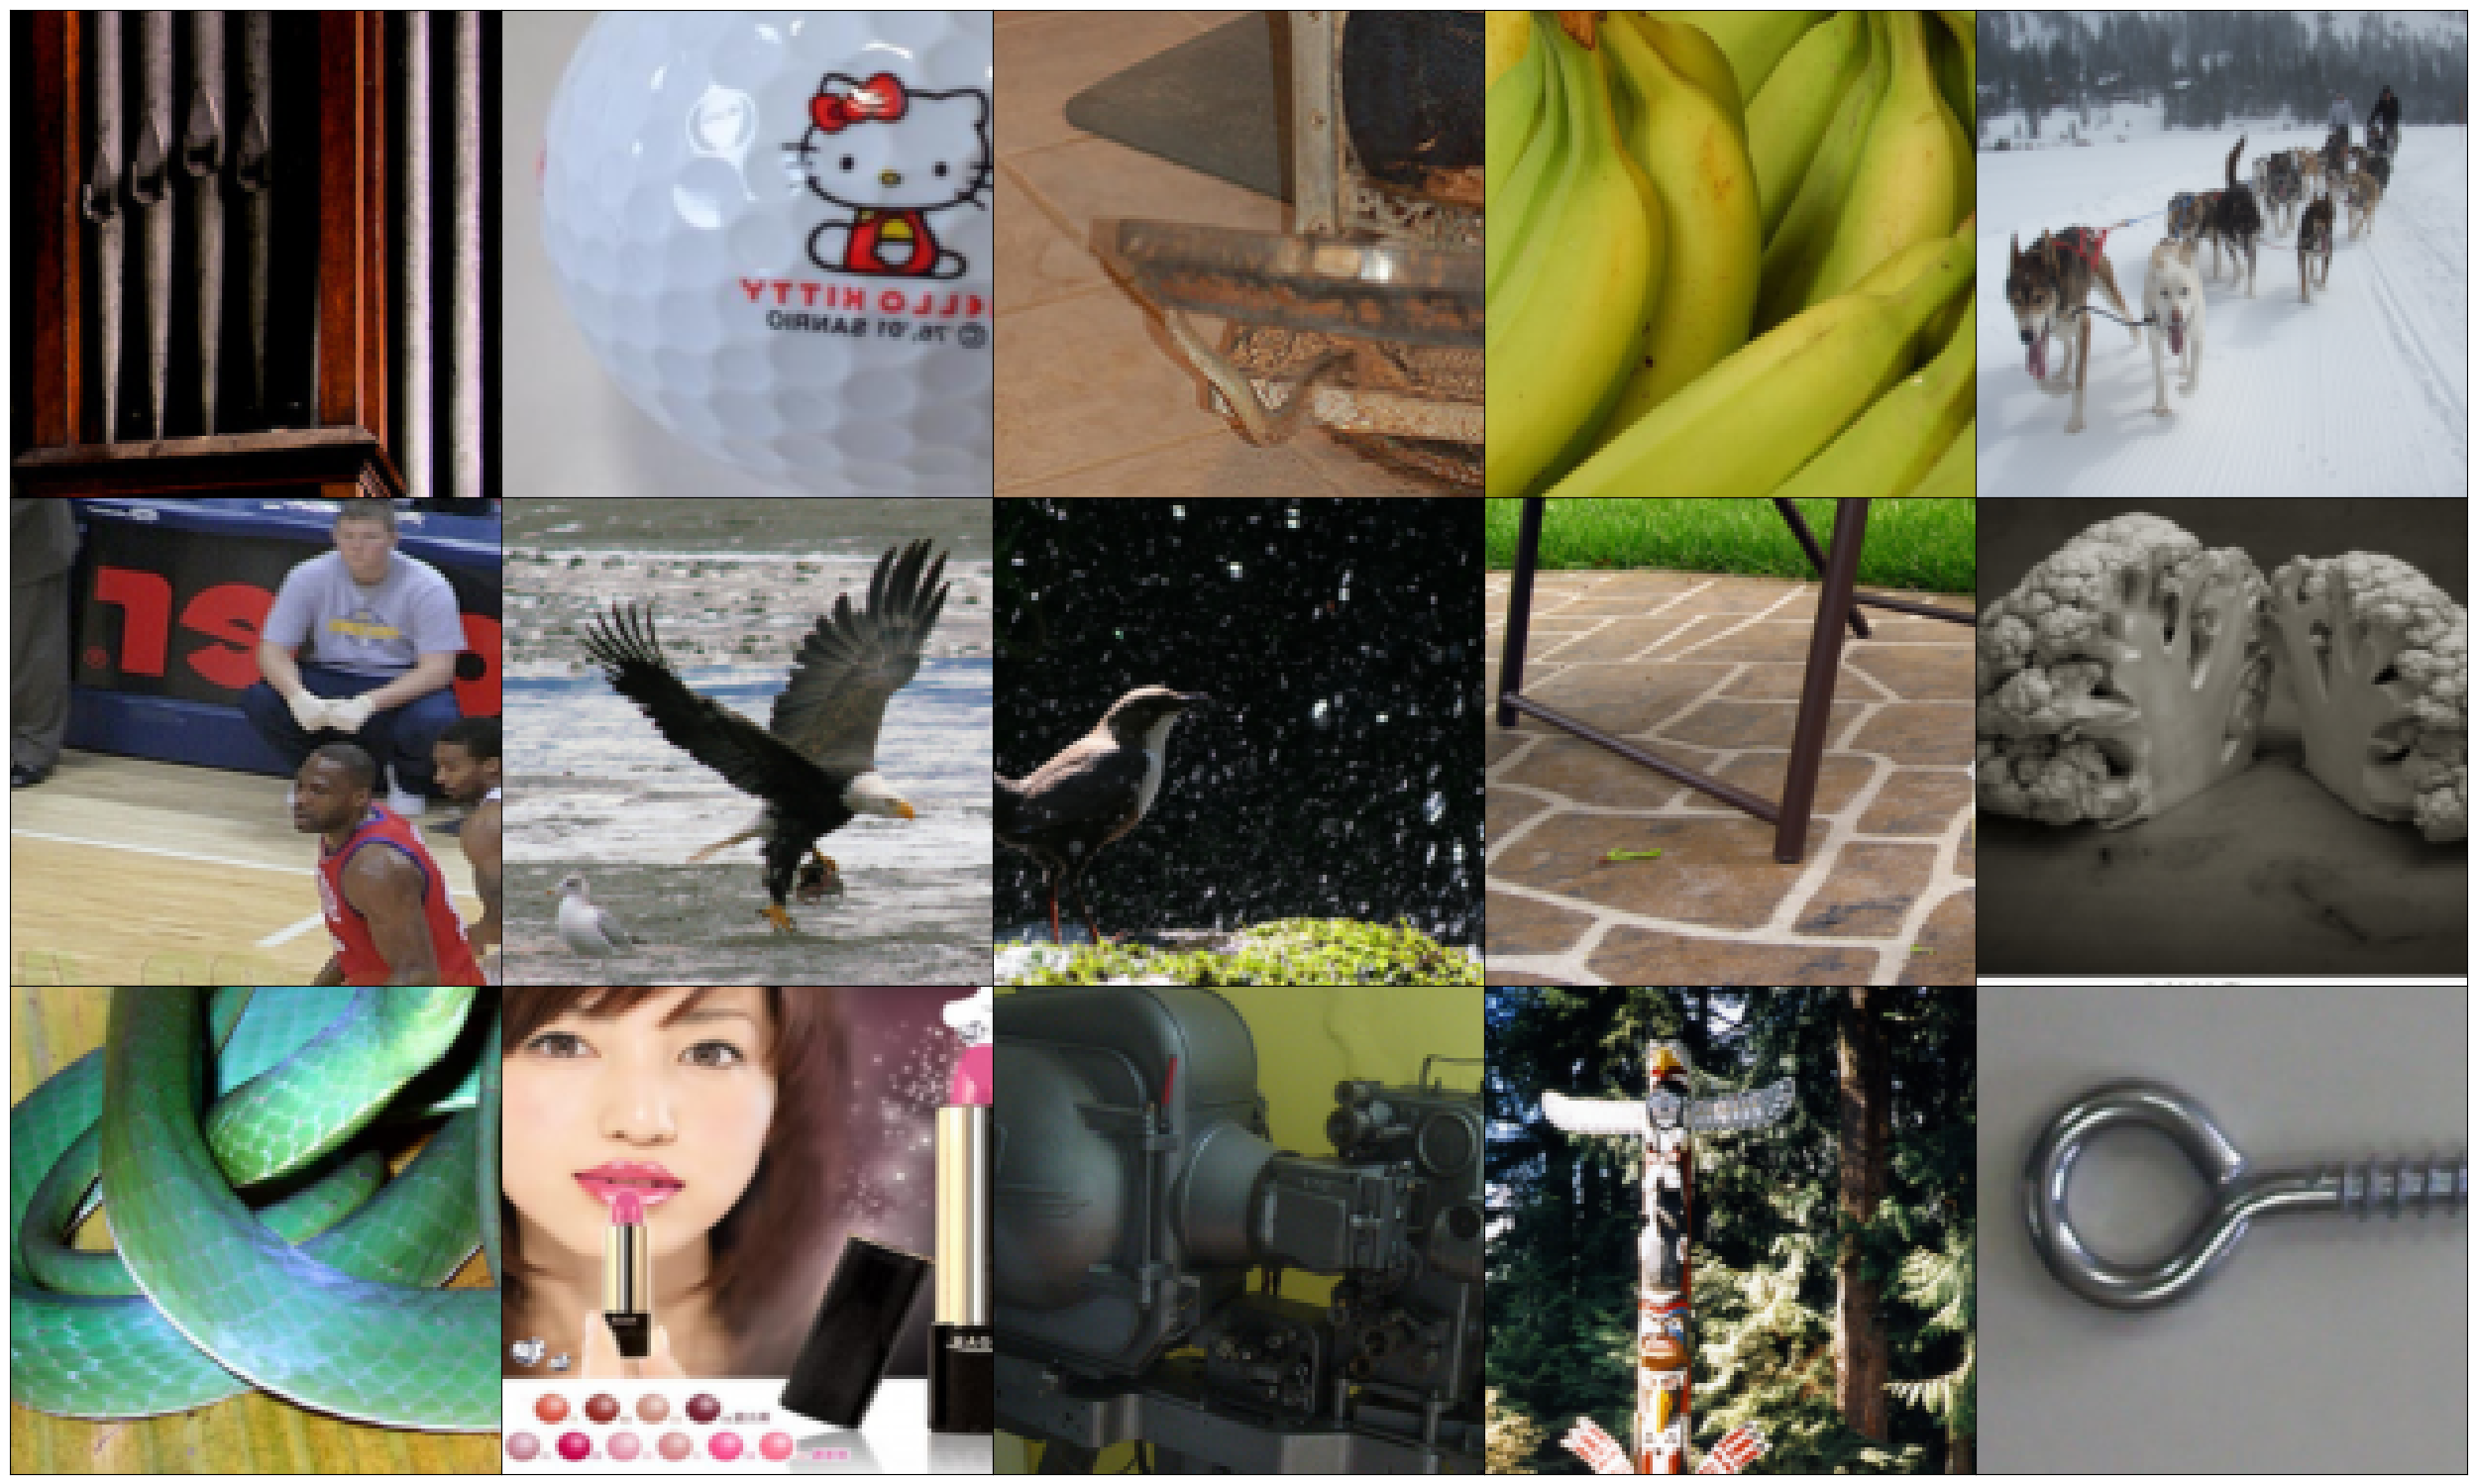
\includegraphics[width=0.5\textwidth]{../../sample_images/imagenet_unnormalized}
        \caption{Example images from the ImageNet dataset randomly cropped and resized to 128x128 pixels and standardized}
        \label{fig:imnet_example_normalized}
    \end{figure}

    \begin{figure}
        \centering
        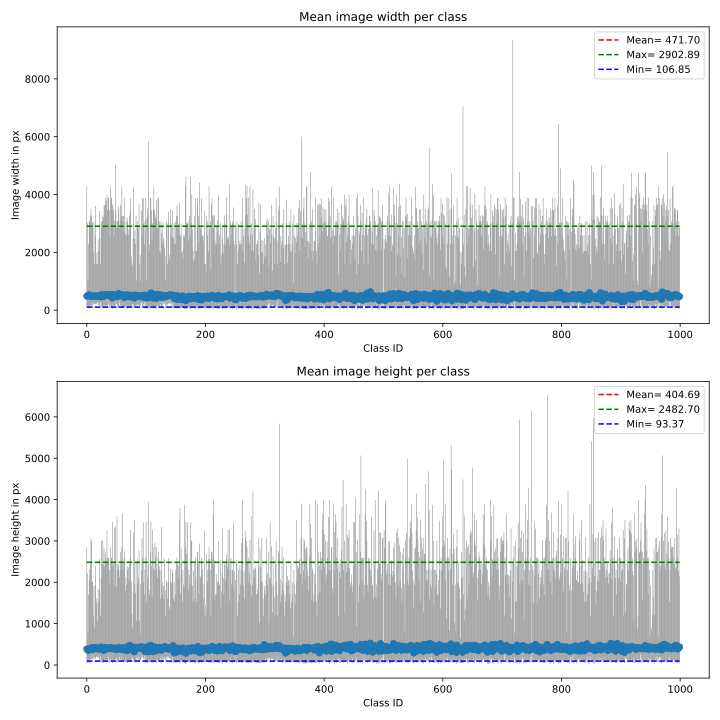
\includegraphics[width=0.5\textwidth]{../../sample_images/imagenet_sizes_errorbar}
        \caption{Image resolution deviations in the ImageNet dataset across classes}
        \label{fig:imnet_sizes_err}
    \end{figure}

    \begin{figure}
        \centering
        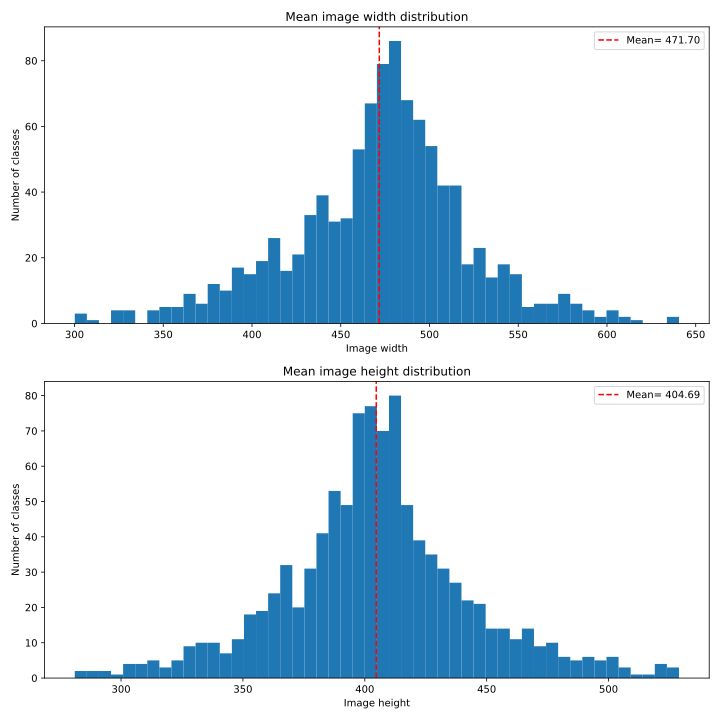
\includegraphics[width=0.5\textwidth]{../../sample_images/imagenet_sizes_histogram}
        \caption{Histogram of image resolutions in the ImageNet dataset}
        \label{fig:imnet_sizes_hist}
    \end{figure}

    \begin{figure}
        \centering
        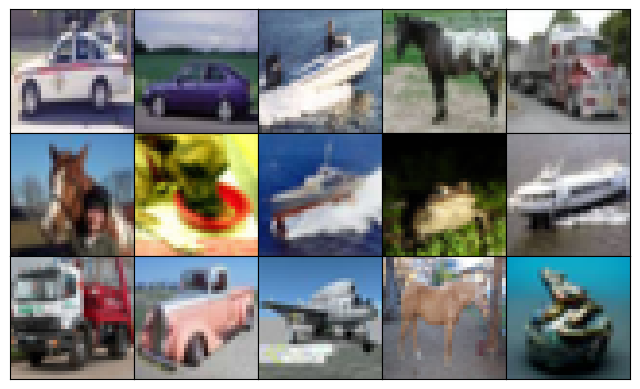
\includegraphics[width=0.5\textwidth]{../../sample_images/cifar_rbatch}
        \caption{Example images from the CIFAR-10 dataset standardized}
        \label{fig:cifar10_example_normalized}
    \end{figure}

    \begin{figure}
        \centering
        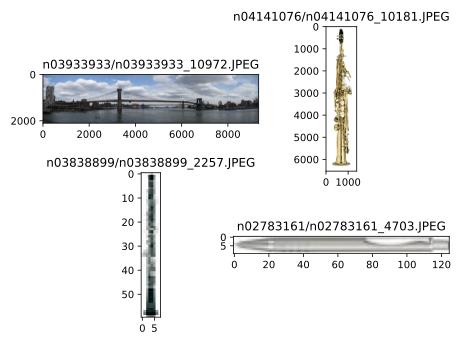
\includegraphics[width=0.5\textwidth]{../../sample_images/optima_shape_examples}
        \caption{Example images from the ImageNet dataset with very unregular resolution ratios}
        \label{fig:optimal_resolution}
    \end{figure}

    \begin{figure}
        \centering
        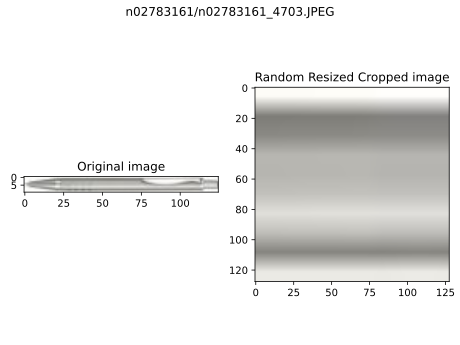
\includegraphics[width=0.5\textwidth]{../../sample_images/random_resized_crop_small}
        \caption{Example image from the ImageNet dataset that is too small}
        \label{fig:small_image}
    \end{figure}